\documentclass{article}
\usepackage{graphicx} % Required for inserting images
\usepackage{listings}
\usepackage{url}
\usepackage{amsmath}
\usepackage{amssymb}
\usepackage{amsfonts}
\usepackage{braket}

\usepackage{listings} %amit AES
\usepackage{nicematrix}
\usepackage{caption}

\usepackage{tikz} %stefan RSA
\usetikzlibrary{fit}
\usepackage{xcolor, soul}

\usepackage[margin=2.5cm]{geometry}
\usepackage{bm}

\usepackage[utf8]{inputenc}
\usepackage[english]{babel}
\usepackage{natbib}

\usepackage{color}
\definecolor{dkgreen}{rgb}{0,0.6,0}
\definecolor{gray}{rgb}{0.5,0.5,0.5}
\definecolor{mauve}{rgb}{0.58,0,0.82}

\newcommand{\round}[1]{\ensuremath{\lfloor#1\rceil}}

\lstset{frame=tb,
    language=Python,
    aboveskip=4mm,
    belowskip=4mm,
    showstringspaces=false,
    columns=flexible,
    basicstyle={\small\ttfamily},
    numbers=none,
    numberstyle=\tiny\color{gray},
    keywordstyle=\color{blue},
    commentstyle=\color{dkgreen},
    stringstyle=\color{mauve},
    breaklines=true,
    breakatwhitespace=true,
    tabsize=4
}

\title{Imperial Project Report \\ 
Cryptography: From Caesar to Quantum}

\author{Tom Ballantyne, Edward Ștefan Bujdei, Amit Paul, Eden Zan}

%\date{November 2024} % ?
\date{\today} %!

\begin{document}

\maketitle

\begin{abstract}
Sending and receiving secret messages safely and securely has been vital for
a useful and functioning cybersystem, and requires some kind of encoding
and decoding mechanism for these messages known as ciphers, for which many
exist under numerous different paradigms. However, developments in quantum
computing within the past 50 years threaten the dependability of most modern
ciphers by potentially making it significantly easier for third parties to
intercept and decode the messages. We have chosen to review and analyse the
candidate ciphers in the domain of \textit{Post-Quantum Cryptography} to
encourage understanding of the future of cybersecurity.
\end{abstract}

\newpage

\tableofcontents

\section{Introduction}
Encryption methods have existed for thousands of years in order to safely
transmit messages from one party to another without 3rd parties
intercepting the data. These vary from rudimentarily designating each
letter in the alphabet with another letter, and replacing each character in
the plaintext with its designated letter, a class of ciphers known as
\textit{monoalphabetic substitution ciphers}, to more complex algorithms
that exploit the hardness of prime factorisation, for example in the RSA
cipher, to ensure the hardness of decrypting the ciphertext. However,
modern encryption methods including the RSA cipher, upon which all of
cybersecurity depends on, have been threatened by known algorithms designed
to run on quantum computers, and while these require a large amount of
computational resources to be efficient, recent and potential future
developments in quantum computing have and will further put these ciphers
at risk. We have elected to research and document candidate future
post-quantum resistant ciphers, ciphers designed to run on classical
computers but be immune to quantum algorithms, suggested by NIST, the
National Institute of Standards and Technology, to assess the safety and
reliability of future communication

\subsection{Caesar Cipher}
One early encryption method was the \textit{Caesar Cipher}, a monoalphabetic 
substitution cipher used by Julius Caesar to securely send messages, which can
be generalised using modular arithmetic.
\medskip

To encrypt the plaintext into ciphertext, each
letter in the plaintext is replaced by a letter that is some fixed number (the
key) of positions down the alphabet. For example a right-shift of 4 would
replace A with E and a left-shift of 3 would replace D with A. If the shift
takes you past the end of the alphabet, you can loop back to the beginning. For
example, a right-shift of 3 on Y would return B. We can therefore generalise 
this cipher as a function $f(x) = x + k (mod n) $, where x is some number value
designated to the letter (for 'b' this would be 2 for instance), k is the key, 
and n is the length of the alphabet.
\medskip

To do this practically, this could be done by alligning two alphabets. The
cipher alphabet is the plain alphabet rotated left or right by a number of
positions. For example, here is a Caesar Cipher that uses a rotation to the
left of three places (equivalent to a rotation to the right of 23):
\medskip

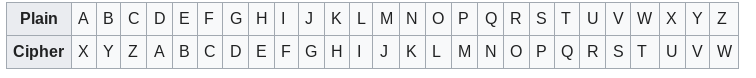
\includegraphics[width = \textwidth]{Screenshot 2024-11-24 22.13.38.png}
\medskip

However, we can also implement this mathematically as suggested above.
This can be seen implemented in the function here:
\medskip
% \includegraphics[width = \textwidth]{Screenshot 2024-11-24 22.51.17.png}
\begin{lstlisting}
def caesar_shift(plaintext: str, keyset: str, key: int) -> str:
    ciphertext = ""
    number_of_keys = len(keyset)

    for char in plaintext:
        if char.lower() in keyset:
            char = char.lower()
            index = keyset.index(char)
            new_index = (index + key) % number_of_keys
            char = keyset[new_index]
            ciphertext += char
        else:
            ciphertext += char
    return ciphertext
\end{lstlisting}
\medskip

The Caesar Cipher was a useful way to protect the transfer of information
thousands of years ago, when it was relatively new. However, because of its
simplicity, people quickly realized that it was very easy to decrypt. This
could be done by a brute force method of simply trying all possible keys
(adding or subtracting all the numbers from 1 to 25) and seeing which one
produced a readable message because the alphabet is so small. As shown
computationally here, but using a different approach to give each letter
numbers as it uses their ASCII value instead of putting them in a list):
\medskip
\begin{lstlisting}
def break_caeser(cypher, keys):
    newplain = ""
    for i in range (0, len(cypher)):
        if ord(cypher[i]) == 32:
            newplain = newplain + chr(32)
        elif ord(cypher[i]) < 97 or ord(cypher[i]) > 122:
            pass
        else:
            num = ord(cypher[i])
            newnum = ((num + keys - 97) % 26) + 97
            newplain = newplain + chr(newnum)
        return newplain      
\end{lstlisting}
This could also be done by trying to deduce the key using frequency analysis,
where common letters and words are compared to the cipher text to see what
shift would be required to produce them and then this key is tested.
The most common letter in the English alphabet is 'e', followed by 't', and 'a'
and so on. Therefore, we could determine which letter is shifted to 'e' for instance
simply by searching for the most common letter, allowing us to find the key for the
caesar cipher.
%something to add here This can be seen implemented computationally here: 
\\
Therefore, the Caesar Cipher no longer has any use in communication security.
However, the encryption step using a key was developed into more complex
ciphers such as the Vigenere Cipher.

\subsection{Vigenere Cipher}
The Vigenere Cipher is a more complicated, \textit{polyalphabetic} substitution
cipher where each letter of the plaintext is encoded with a different Caesar
Cipher, determined by the corresponding letter of another word, the key. it is
not simply monoalphabetic as the same letter in two different positions may be
ciphered to different letters. the plaintext is split into sections each the
length of the key. The first letter of the section will be encoded by a caesar
Cipher shift of the numerical value in the alphabet of the first letter in the
key. This continues in each section. For example, if the first letter of the
plaintext in A and the first letter of the key is E then A will undergo a
left-shift of 5 (as E is the 5th letter in the alphabet).
\medskip

To do this computationally the plaintext should be split into sections (each
the same length as the key length). This can be done by keeping a counter that
increments each time a letter is Caesar shifted and if it gets larger than the
length of the keyword will go back to 0. This counter can be used as the index
to use the correct letter of the keyword to use for the Caesar shift. This can
be seen being implemented here:\medskip

% \includegraphics[width = \textwidth]{Screenshot 2024-11-24 23.44.31.png}
\begin{lstlisting}
def vigenere_cipher(plaintext: str, keyword: str) -> str:
    ciphertext = ""
    current_cipher_index = 0
    length_of_keyword = len(keyword)

    for char in plaintext:
        if char.lower() in alphabet:
            if current_cipher_index > length_of_keyword - 1:
                current_cipher_index = 0
            local_key = alphabet.index(keyword[current_cipher_index].lower())
            ciphertext += caesar_shift(char, alphabet, local_key)
            current_cipher_index += 1
        else:
            ciphertext += char

    return ciphertext
\end{lstlisting}
\medskip
This method of encryption is much more secure than the Caesar Cipher as each
letter could be shifted by any of the 26 letters so without the key it is very
hard to work out how to decrypt each letter. However, due to the repetitive
nature of the key it can sometimes be possible to break this cipher.\medskip

One way this can be done by looking for repeated sections in the ciphertext and
seeing how far apart they are from each other. The key length can then be
assumed to be a factor of this distance. For example in the following
ciphertext:
\medskip

\[\bm{CSASTP}KVSIQUTGQU\bm{CSASTP}IUAQJB\]
\medskip
The substring "CSASTP" is 16 letters apart. Therefore, it can be assumed that
these repeated segments represent the same plaintext segments and so the key
length is a factor of 16 (16,8,4,2,1). This is easier to implement with longer
plaintexts as there are likely to be more repeated segments. The key length can
then be guessed by looking at common factors of the distances between all the
repeated segments. This method to guess the key length is known as 'Kasiski
analysis' \cite{kasiski} which we can see implemented here:
\medskip

\begin{lstlisting}
def kasiski_analyser(ciphertext: str) -> list[int]:
    string_to_analyse = ""
    for char in ciphertext:
        if char != " ":
            string_to_analyse += char # remove spaces

    repeated_substrings = {} #substring: [positions]

    for substring_length in range(3, 12):
        for i in range(len(string_to_analyse) - substring_length - 1):
            potential_repeat = string_to_analyse[i:i+substring_length]

            positions = []
            index = 0
            while index < len(string_to_analyse):
                index = string_to_analyse.find(potential_repeat, index)
                if index == -1:
                    break
                positions.append(index)
                index += substring_length

            if len(positions) > 1 and potential_repeat not in repeated_substrings:
                if positions[0] % substring_length == positions[1] % substring_length:
                    repeated_substrings[potential_repeat] = positions

    distances = []
    for sub in repeated_substrings:
        distances.append(repeated_substrings[sub][1] - repeated_substrings[sub][0])

    d_factors = []
    for distance in distances:
        d_factors += factors(distance)
        # factors(n) returns a set of the factors of n

    # remove 1
    d_factors = [num for num in d_factors if num != 1]
    # sort into frequency
    d_factors = [i for items, c in Counter(d_factors).most_common() for i in [items] * c]
    # remove duplicates
    d_factors = list(dict.fromkeys(d_factors))
    # adds back one if the list is empty
    d_factors = [1] if d_factors == [] else d_factors

    return distances_factors
\end{lstlisting}
However, kasiski analysis has a higher liklihood to fail if the ciphertext is 
smaller, as it depends on repeating substrings, which are less likely to be 
present in short ciphertexts.
\medskip

Once the length of the key is guessed, the ciphertext can be split into many
columns, with each column corresponding to one letter of the key. Frequency
analysis can then  be used on each column where the most common letters in that
column are compared to the most common letters in the english language to try
and find the value of the Caesar shift in that column.
%This method (using both frequency analysis and Kasiski analysis) can be seen implemented here:
\medskip

Overall, the Caesar Cipher is a very primitive cipher that is very easy to
crack. The Vigenere cipher is more advanced but for longer plaintexts can
almost always be solved by using frequency analysis. Therefore, neither of
these methods are used in modern day communication.

\subsection{AES and Symmetrical Encryption}
AES is a symmetrical cipher, meaning that the key to encode information is identical to the key to decode the ciphertext.
AES works as a block cipher with a plain text size of 128 bits and a key size of 128/192/256 bits. The plain text, which we shall refer to as the "state", is separated into a block of 4 by 4 bytes. We can then apply a series of functions in order to the state, resulting in a cipher text.
\\
AES works on 2 fundamental rules:
\begin{itemize}
    \item Diffusion
    \item Confusion
    \medskip
\end{itemize}
Confusion is all about complicating the relationship between the key and the cipher text. 1 bit of the cipher text should depend on more than 1 bit of the key. Diffusion is all about changing the statistical structure of the cipher text, for every bit changed in the key, approximately half of the bits should change for the cipher.
\subsubsection{Key expansion}
Firstly, the original key is expanded into multiple round keys depending on the size of the original key. The size of the original key also determines how many rounds of transformations there will be.\medskip
\begin{center}
\begin{NiceTabular}{|c|c|c|}[name=AESgrid]

\hline
AES-128&AES-192&AES-256\\  
11 round keys& 13 round keys& 15 round keys\\ 
10 rounds&12 rounds&14 rounds\\ 
\hline

\end{NiceTabular}
\end{center}
\medskip
As seen from the figure, AES-128 consists of 11 round keys and a total of 10 rounds. To generate these round keys, we are going to concatenate the bytes in each of the columns from the state, this results in 4 words. 
\begin{center}
\begin{NiceTabular}{|c|c|c|c|}[name=State]

\hline
\(B_{0}\)&\(B_{4}\)&\(B_{8}\)&\(B_{12}\)\\  \hline
\(B_{1}\)&\(B_{5}\)&\(B_{9}\)&\(B_{13}\)\\ \hline
\(B_{2}\)&\(B_{6}\)&\(B_{10}\)&\(B_{14}\)\\ \hline
\(B_{3}\)&\(B_{7}\)&\(B_{11}\)&\(B_{15}\)\\ \hline

\end{NiceTabular}
\end{center}
\begin{center}
$\downarrow$
\end{center}
\begin{center}
\begin{NiceTabular}{|c|c|c|c|}[name=Word-array]

\hline
\(W_{0}\)&\(W_{1}\)&\(W_{2}\)&\(W_{3}\)\\
\hline

\end{NiceTabular}
\end{center}
Hence, getting the first round key. For the subsequent round keys, you are going to input the last word into a g function. This g function will then perform some operations to this input, returning a completely different word. These operations are as follows:
\begin{itemize}

    \item A one byte left circular shift. This means the bytes of the word are all moved 1 place to the left, the first byte is moved at the end position.
    
\end{itemize}
\begin{center}
\begin{NiceTabular}{|c|c|c|c|}[name=Word_Bytes]
\hline
\(B_{0}\)&\(B_{1}\)&\(B_{2}\)&\(B_{3}\)\\
\hline
\end{NiceTabular}
\end{center}
\begin{center}
$\downarrow$
\end{center}
\begin{center}
\begin{NiceTabular}{|c|c|c|c|}[name=Shifted_Bytes]
\hline
\(B_{1}\)&\(B_{2}\)&\(B_{3}\)&\(B_{0}\)\\  
\hline
\end{NiceTabular}
\end{center}
 . . .


\subsection{RSA and Public-Key Encryption}
RSA is an assymetric modern cipher that is currently in use, which uses the
difficulty of prime factorisation to efficiently encrypt text.
A \textit{symmetric} cipher can be seen as follows, in order to demonstrate the 
flaws of this paradigm.
\medskip
We will call the sender of a message Alice and the receiver Bob.
All classical ciphers rely on a key that both Alice and Bob know, which is 
in practice stored locally.
This has some major disadvantages:

\begin{enumerate}
   \item Alice and Bob need to meet to decide on a key
   %\item It is easy to find the key 
   \item If someone else finds the key, they will be able to:

   \begin{itemize}
      \item Read all encrypted messages
      \item Send messages pretending to be Alice or Bob
   \end{itemize}

   %\item Alice and Bob need to meet to decide a key
\end{enumerate}

Where an operation is described as \textit{\lq{}easy\rq{}} it has time and
space complexities with less than exponential growth.

Current Cryptography relies on a different approach, instead of Alice and Bob
using the key, Alice locks her ciphertext with Bob's lock. So no-one (not even
Alice) can unlock the message except Bob. This needs a lock that is extremely
hard to break (to unlock without the private key) but very easy to unlock for
Bob (the intended recipient*), as he of course has the key to his own lock.

We will call this "lock" a \textit{public key} and the key that is secret a
\textit{private key}. A message can be encrypted by anyone using the public key
and can only be decrypted by the person with the private key.
The algorithm for generating the public and private keys should make it easy to:
\begin{itemize}
   \item	Generate public and private keys
   \item Decipher the ciphertext with the private key
\end{itemize}

But difficult to decipher the ciphertext without the private key
This is called a \textit{trapdoor algorithm}.

\subsubsection{Key Generation, Encryption and Decryption}
We assume that there is no easy algorithm for factoring large primes.
\begin{itemize}

   \item To encrypt a message:
      $ C \equiv M^e \mod n $

   \item To decrypt a message:
      $ M \equiv C^d \mod n $

\end{itemize}

Where the following should be explained before the formula:
C is the ciphertext (the encrypted message)
M is the message (as an number)

We generate numbers n, e, and d such that:
\begin{itemize}
   \item The values are computable (so the sender can encrypt their message)
   \item It must be difficult to calculate d given e, n and C (as the latter will all be publicly accessible and d would allow eavesdroppers to read the message)
   \item The message can be decrypted only by knowing d (so an eavesdropper can not read the message)
   \item $d =$ the private key
   \item $e =$ part of the public key
   \item $n =$ part of the public key

   \item $n$ is chosen to be the product of 2 primes: p and q
   \item The difference of $p$ and $q$ should be high so that checking numbers near $\sqrt{n}$ (which is easy to calculate) does not reveal $p$ and $q$
\end{itemize}

\[
   n = pq 
\]

We define $\phi(n)$ as the 'Euler Totient Function' of $n$, which is the number of numbers less than $n$ which are coprime to $n$.
Since $n$ has a known factorisation (to the users of the key, but unknown to the third parties), we are able to efficiently 
calculate this as $(p-1)(q-1)$.

Then select d to be a coprime to $\phi(n)$.

Then select $e$ such that:

\[
   ed \equiv 1\mod\phi(n)
\]
This ensures that e and d are multiplicative inverses of eachother $\mod n$, allowing us to use them as our private and public keys.

For example, let $p$ and $q$ $= 5$ and $31$ respectively. Then $n = pq = 5 * 31
= 155$. In reality these numbers would be very large, though for the sake of demonstration we have ignored this.
We can then choose $d$ to be $7$, as $7$ is coprime to $(5-1)(31-1)$, or $120$. (It happens to be coprime to every
number, as it is prime itself). Then we can choose $e$ as $103$, as $103 * 7 \equiv 1 \mod\phi(n)$.
\\
Using 7 and 103 as our private and public keys, we can encrypt, for example,
the letter 'a', with ASCII value $97$, as $97^7 \mod 155$, equal to $78$, and
decrypt this as $78^{103}\mod 155$, which is equal to 97.

\subsubsection{The Hardness of Prime Factorisation}

We defined $\phi(x)$ as a function that returns the number of integers less
than $x$ that are coprime to $x$ (they share no prime factors). For example:
\begin{center}

\[\phi(3)=2\]
\begin{NiceTabular}{*3{c}}[name = Three]
1&2&3\\
	\CodeAfter
		\tikz \node [fill=green, opacity = 0.3, rounded corners, fit = (Three-1-1)(Three-1-2)]{};
\end{NiceTabular}


\[\phi(7)=6\]
\begin{NiceTabular}{*7{c}}[name = Seven]
1&2&3&4&5&6&7\\
	\CodeAfter
		\tikz \node [fill=green, opacity = 0.3, rounded corners, fit = (Seven-1-1)(Seven-1-6)]{};
\end{NiceTabular}


\end{center}
Generally, where \(p\) is a prime: \(\phi(p) \equiv p-1\) because p is coprime
to all the positive integers lower than it and there are $x-1$ positive
integers less than $x$.
\begin{center}
\[\phi(p) \equiv p-1\]
\[
\underbrace{1\thickspace2\thickspace3\thickspace\ldots\thickspace}_\text{$p-1$ numbers} p
\]

\[\phi(7\times3)\]
\begin{NiceTabular}{*7{c}}[name = 21]
1&2&3&4&5&6&7\\
8&9&10&11&12&13&14\\
15&16&17&18&19&20&\thickspace\\
	\CodeAfter 
		\tikz\node[fill=red,opacity=0.3,fit=(21-1-7)(21-2-7),rounded corners]{};
		\tikz\node[draw,dashed,fit=(21-1-3),rounded corners]{};
		\tikz\node[draw,dashed,fit=(21-1-6),rounded corners]{};
		\tikz\node[draw,dashed,fit=(21-2-2),rounded corners]{};
		\tikz\node[draw,dashed,fit=(21-2-5),rounded corners]{};
		\tikz\node[draw,dashed,fit=(21-3-1),rounded corners]{};
		\tikz\node[draw,dashed,fit=(21-3-4),rounded corners]{};
\end{NiceTabular}\\ 

\begin{NiceTabular}{*2{c}}[name = 21key]
multiple of 7& multiple of 3\\
\CodeAfter \tikz\node[fill = red, opacity=.3,rounded corners, fit = (21key-1-1)]{};
\tikz\node[draw, dashed, rounded corners, fit = (21key-1-2)]{};
\end{NiceTabular}\\ 

\end{center}

This is the grid for \(\phi(7)\) with an aditional 3 rows. Notice that all the
multiples of 7 are in the last column and there is a single multiple of 3 in
each column. This means that for each coprime to 7, there are 2 less than 21
that are also coprime to 3 (numbers coprime to 3 and 7 are coprime to 21).

Euclid's algorithm finds the Greatest Common Divisor (GCD) of 2 numbers. If the
GCD of 2 numbers is 1, then they are coprime.  The result of a division is
given as quotient "r" remainder.
For example, to find \(GCD(50,15)\)
\[
50 \div 15 = 3 \text{ r } 5\]
\[
   15 \div 5 = 3 \text{  r  } 0
\]
When the remainder is 0, the divisor of the last division is the greatest
common divisor so \(GCD(50,15) = 5\)\\

Or, to find \(GCD(50,13)\)
\[50 \div 15 = 3 \text{  r  } 11\]
\[13 \div 11 = 1\text{  r  }2\]
\[11 \div 2 = 5\text{  r  }1\]
\[2 \div 1 = 2\text{  r  }0\ \text{ so 1 is the greatest common divisor}\]
\[GCD(50,13) = 1 \text{  so  } 50 \text{ and } 13 \text{ are coprimes}\]

To break RSA we must find the prime factors of N.


\subsection{Shor's Algorithm}
\subsubsection{Quantum Computers}
   A quantum computer is a computer that exploits quantum mechanical phenomena.
   It takes advantage of the quantum world’s properties of very small amounts
   of physical matter, such as electrons, exhibiting both properties of
   particles and waves to enable a bit of data to act as both a 0 and 1 at the
   same time (known as a qubit) to make calculations much quicker and more
   efficient than would be possible on a conventional computer. 
   \medskip

   Quantum mechanics is the study of matter and its interactions with energy on
   the scale of atomic and subatomic particles. It explains that extremely
   small objects exhibit both properties of particles and waves- known as
   wave-particle duality. This can be seen when electrons are fired from an
   electron beam gun, through a double-slit, onto a screen and an interference
   pattern is produced, similar to one seen when a light wave is passed through
   a double-slit. This shows that electrons are exhibiting properties of waves,
   passing through both slits simultaneously, diffracting and interfering to
   produce an interference patt/ern. This pattern is the result of
   superposition, where the electron is in a superposition of going through
   both slits at the same time and the interference between these two states
   produces the interference pattern. However, when you try to observe the
   electron passing through the double slit, the electron stops acting as a
   wave and acts as a single particle and the interference pattern disappears,
   forming two heaps of electrons behind each slit. This shows how electrons
   (and other small particles) can be in a superposition of states and act as
   both particles and waves. The electrons can also influence the quantum state
   of other electrons through entanglement where  the quantum state of one
   electron is tied to those of nearby electrons, even if they are later
   separated by considerable distances.
   \medskip

   Just like how the electrons in the double-slit experiment can be in a
   superposition of passing through both slits, qubits in a quantum computer
   can be in a superposition of being 0 and 1 at the same time. Therefore, when
   measuring qubits, the result is a probabilistic output of a classical bit.
   This allows quantum computers to process a large amount of possibilities in
   parallel, making them much faster than conventional computers. In addition,
   qubits (like electrons) can become entangled, so that the state of one qubit
   is directly linked to others even if they are separated. This creates
   correlations between qubits that are stronger than what classical physics
   allows. Entanglement is used in quantum computing to link qubits in such a
   way that the information in the system as a whole is processed more
   efficiently. Quantum computers also use quantum interference to amplify the
   probability of correct answers while canceling out incorrect ones. This
   process allows quantum computers to narrow down potential solutions in a way
   that is much more efficient than classical computation.
   \medskip

   Currently, quantum computers are not yet practical for the real world as it
   has proven difficult to engineer and control high-quality qubits, meaning it
   has not yet been possible to built quantum computers with many qubits.
   Qubits also can suffer quantum decoherence, leading to noise in calculations
   if they're not sufficiently isolated from their environment. However,
   national governments have invested heavily in trying to develop quantum
   computers that can control many qubits with less noise and therefore lower
   error rates. Although the future creation of computers will hold lots of
   benefits as calculations can be done much more efficiently, they also hold
   some dangers for this same reason. One of the main dangers in encryption.
   This is because current encryption techniques rely on the difficulty of
   specific mathematical problems, such as factoring large numbers or solving
   discrete logarithms. These problems are intractable for conventional
   computers, however quantum computers can crack these problems exponentially
   faster than conventional computers. Therefore, ciphers resistant to attacks
   from quantum computers must be built for future usage.

\subsubsection{Prime Factorisation}
   %As discussed in the section on RSA, classical computers struggle with
   %step n. % dunno how stefan will number this yet.
   %Classical computers can reduce prime factorisation to order-finding,
   %which is, when factorising $N \in \mathbb{N}$ using a random $a \in \mathbb{N}$
   %such that $2 \le a < N$, finding $r \in \mathbb{N}$
   %such that $a^r \equiv 1 \mod{N}$ and $\gcd(a, N) \neq 1$.
   %Shor's algorithm is able to find $r$ much quicker than classical
   %computers using the \textit{Quantum Fourier Transform} (QFT).
   %\medskip
   %The QFT is the quantum analogue of the discrete Fourier transform (DFT),
   %used to analyse periodic funtctions by mapping between time and
   %frequency representations. In brief, the DFT takes an input vector
   %$(x_0, x_1, \ldots, x_{N-1}) \in \mathbb{C}^N$ and returns an
   %output vector $(y_0, y_1, \ldots, y_{N-1}) \in \mathbb{C}^N$ where:
   %\[y_k = \sum_{j=0}^{N-1}x_j\exp\left( -\frac{2\pi i j k}{N} \right)   \]
   %However, the QFT performs roughly the same operation, but in the quantum
   %state $\ket{x} = \sum_{i=0}^{N-1}x_i\ket{i}$, and outputs another
   %quantum state $\ket{y} = \sum_{i=0}^{N-1}y_i\ket{i}$ where:
   %\[y_k = \frac{1}{\sqrt{N}}\sum_{j=0}^{N-1}x_j\exp\left( \frac{2\pi i j k}{N} \right)\]
   %assuming $N = 2^n$ for ease of comparison.
   %\medskip
   %The QFT is then utilised for \textit{Quantum Phase Estimation} (QPE), which
   %estimates the phase, or eigenvalue, of a quantum system
   %
   %%Shor's algorithm is able to utilise the functionality of quantum
   %%computers to 

   Shor's algorithm is one of the most groundbreaking discoveries
   in quantum computation, allowing us to factorise integers
   more efficiently. As discussed in the section on RSA, the problem
   of prime factorisation is reducible to finding the period $r$ of a 
   function $f(x) = a^x \mod{N}$, where $a$ is a random number and 
   $N$ is the number to be factorised (so that $f(x) = f(x+r)$). For
   simplicity, we will only consider the case where $r$ exactly divides
   the number of points $N = 2^n$, or simply that $N/r = m$ where $m$
   is an integer (for more general cases, and overall more detail see
   Shor, 1997).
   \medskip
   We then need to prepare a register in the equal superposition state
   and another which stores the function $f(x)$ building the total state:
   \[\frac{1}{\sqrt{2^n}}\sum_{x=0}^{2^n-1}\ket{x}\ket{f(x)}\]
   The modular exponentiation function can be computed efficiently in 
   both classical and quantum computers, but \textit{quantum parallelism}
   allows $f(x)$ to be computed for all $x$ in a single run. In addition
   after function evaluation, the registers are \textit{entangled}. Though
   we cannot access directly the values of $f(x)$, it collapses into a single
   state $\ket{f(x_0)}$ after measuring the second register. Therefore, the
   quantum computer wave function becomes:
   \[\frac{1}{\sqrt{m}}\sum_{j=0}^{m-1}\ket{x_0+jr}\ket{f(x_0)}   (0 \le x_0 < r-1)\]
   where $m = N/r$ is the number of x values such that $f(x) = f(x_0)$.
   Since $f(x)$ has period $r$, it follows that $f(x_0) = f(x_0 + r)
   = f(x_0 + 2r) = \ldots = f(x_0 + (m-1)r)$. We can then proceed to
   ignore the second register, as it has been factorised and no longer
   relevant to us. It can be checked that a quantum Fourier transform
   of the first register gives the state:
   \[\frac{1}{\sqrt{r}}\sum_{k=0}^{r-1}\exp\left(\frac{2\pi x_0 k}{r}\right)\ket{k\frac{N}{r}}\]
   which shows that \textit{quantum interference} has selected a few
   specific frequencies. A quantum measurement of the wave function
   above gives one of the $r$ outcomes $kN/r \text{     } (k = 0, 1, \ldots, r-1)$
   with equal probability. Therefore, denoting $c$ as the measured
   value, we have that $c/N = \lambda/r$ where $\lambda$ is an unkown
   integer. Therefore, if we reduce $c/N$ to an irreducible fraction,
   we will be left with $\lambda$ and $r$, which number theory informs
   will occur with a probability at least $\frac{1}{\log\log r}$,
   otherwise the algorithm fails and must be repeated. The algorithm,
   however, should succeed with a probability arbitrarily close to one
   after a number of runs $O(\log \log r)$.
   \medskip
   \\
   Shor's algorithm can execute very efficiently on a quantum computer
   with a sufficient number of bits, meaning it poses a major threat
   to all prime-factorisation based cryptosystems (as well as systems
   with other bases, such as those based on elliptic curves).


\section{Methods}
Due to the security concerns of modern cryptosystems posed by quantum
computers, there have been numerous attempts to develop new systems that are
resistant to quantum algorithms, yet are still able to run on classical
computers. Of these, NIST have identified four algorithms to be standardised.

\subsection{Principles for Quantum-Resistant Cipher Development}
Ciphers currently in use are based around prime factorisation, discrete
logarithms and elliptic curves, all of which have an efficient quantum
algorithm due to Peter Shor. Therefore, cryptographers have used different
mathematical principles for developing future ciphers.

\subsubsection{Worst-Case Lattice Problems}
\subsubsection{Learning With Errors}
Suppose we are to recover a secret $\bm{s} \in \mathbb{Z}^{n}_{q}$, meaning $s$ is an $n$-length vector of integers mod $q$.
We are given that, for example:
\[ 5s_{1} + 3s_{2} + 10s_{3} = 6 \mod{17} \] 
\[ 12s_{1} + 9s_{2} + 4s_{3} = 14 \mod{17} \] 
\[ 13s_{1} + 3s_{2} + 8s_{3} = 5 \mod{17} \] 
For classical computers, this is trivially easy to solve using Gaussian
elimination, where all calculations are performed modulo 17. We can represent
this system as a matrix as follows:
\[
\left(\begin{array}{@{}ccc|c@{}}
   5 & 3 & 10 & 6 \\
   12 & 9 & 4 & 14 \\
   13 & 3 & 8 & 5
\end{array}\right)
\]
This is then reducible to the following matrix:
\[
\left(\begin{array}{@{}ccc|c@{}}
   1 & 0 & 0 & 5 \\
   0 & 1 & 0 & 16 \\
   0 & 0 & 0 & 12
\end{array}\right)
\]
This gives us the solution $s = \begin{pmatrix} 5 \\ 16 \\ 12 \end{pmatrix}$. \\
In fact, the time complexity of Gaussian elimination is $O(n^{3})$, where $n$
is the number of equations and variables, meaning simultaneous equations can be
solved efficiently in \textit{polynomial time}, which is relatively quickly
compared to other algorithms.
\\

However, we can make solving simultaneous equations significantly harder to solve by adding some \textit{error}.
Suppose instead we are to recover secret $\bm{s} \in \mathbb{Z}^{n}_{q}$ and are given:
\[ 5s_{1} + 3s_{2} + 10s_{3} \approx 6 \mod{17} \] 
\[ 12s_{1} + 9s_{2} + 4s_{3} \approx 14 \mod{17} \] 
\[ 13s_{1} + 3s_{2} + 8s_{3} \approx 5 \mod{17} \] 
\[\vdots\]
where each equation is correct up to some small additive error, say $\pm 2$. If
we try to use Gaussian elimination on a system of equations with error, then by
performing operations on combinations of these equations we begin to amplify
the error on our equations.
\medskip

LWE is used as the basis for many PQR ciphers as there are strong reasons to believe that it is secure.
\\
One reason is that the best known algorithm has time complexity $2^{O(n)}$, even making use of quantum computers.
\\
Another reason is that it is an extension of the \textit{learning parity with
noise} problem. The LPN problem is a special case of the LWE problem where
equations are done modulo 2, so that the error can only be 1, occuring with
probability $\epsilon$. This is already an widely researched problem in learning
theory that is widely believed to be hard, and allowing the modulus to be even
greater than 2 increases the hardness. Furthermore, any algorithmic progress
with LPN would be a breakthrough in coding theory, as it can be formulated as
the problem of decoding from random linear binary codes.
\\
The most significant reason is due to the ties LWE has with lattice problems.
For example, we can assume that G$_{AP}$SVP, the decision version of the
shortest vectors problem, is hard to approximate even with a 'hint' of a short
basis, or we can assume that G$_{AP}$SVP or SIVP, the shortest independent
vectors problem, is hard to approximate within polynomial factors even using
quantum computers. Both of these assumptions we have enough reasonable evidence
to believe.
\\
For these reasons, we can trust the security of cryptosystems that use the principles
of LWE against both classical and quantum algorithms.

\subsection{Auxilliary Efficiency Algorithms}
\subsubsection{Fast Fourier Transform}
\subsubsection{Extended Euclidean Algorithm}

\section{NIST-approved Quantum-Resistant Ciphers}
\subsection{CRYSTALS Kyber}
Kyber is a post-quantum cryptosystem which uses the LWE problem to safely establish a shared secret between two parties.
It revolves around using lattices of polynomials to encrypt and decrypt messages.

\subsubsection{Key Generation}
The key generation algorithm has a series of parameters:
\begin{itemize}
   \item $n$, the (maximum) degree of the polynomials;
   \item $k$, the order of the lattices;
   \item $q$, the modulus, which must be prime;
   %\item $\eta$, which dictates the shape of the binomial distribution from which error values can be generated.
\end{itemize}
We can now define $s$ and $e$ as a two $k \times 1$ order matrices of polynomials with degree $n$ and small coefficients,
chosen through a binomial distribution.
%\\
Then we define $A$ as a $k \times k$ order matrix with elements of polynomials with degree $n$ and random coefficients which are lesser than $q$.
%\\
Finally, we define $t = As + e$, and can output $(A, t)$ as our public key and keep $s$ safe as our secret key.
In the calculation of t, all operations are performed modulo q, and then modulo $x^{n} + 1$, to ensure that all coefficients remain lesser than $q$,
and that the order of the resulting polynomials have degree lesser than $n$.
%\\
The addition error polynomial $e$ ensures that we cannot easily find $s$ simply from $A$ and $t$.
\medskip
We may, for example, define $A$, $s$, and $e$ as follows, using parameters $n$ = 4, $k$ = 2, and $q$ = 91:
\[ A = \begin{pmatrix}
         59x^4 + 64x^3 + 7x^2 + 16x + 46 & 49x^4 + 51x^3 + 73x^2 + 46x + 22 \\
         66x^4 + 65x^3 + 36x^2 + 34x + 54 & 28x^4 + x^3 + 76x^2 + 65x + 87
       \end{pmatrix}
\]

\[ s = \begin{pmatrix}
   2x^4 + x^3 + 2x - 1 \\
   -x^3 - x^2 + 1
       \end{pmatrix}
\]

\[
   e = \begin{pmatrix}
      -x^4 + 2x^2 + x + 2 \\
      -x^4 -x^2
       \end{pmatrix}
\]

It then follows that under modulo 91 and modulo $x^4 + 1$:
\[
   t = \begin{pmatrix}
      24x^3 + 46x^2 + 79x + 26 \\
      54x^3 + 30x^2 + 69x + 12
       \end{pmatrix}
\]
We publicise $(A, t)$ as our public key and keep secret $s$ as our secret key.

\subsubsection{Encryption}
The encryption algorithms transforms a message, in the form of an integer, and a public key, which is a pair of matrices of polynomials,
into a matrix of polynomials paired with a single polynomial as the ciphertext.
\medskip
The first step is to convert our integer message $M$ into a polynomial $M_{b}$. We do this by taking the binary representation of the polynomial,
then taking each single digit as a coefficient in a polynomial. For example, we convert the integer $13 = 8 + 4 + 1$ into the polynomial
$(1)x^{3} + (1)x^{2} + (0)x^{3} + 1$, or simply $x^{3} + x^{2} + 1$.
Then, we multiply each coefficient by $\round{q/2}$, the nearest integer to $q/2$, to generate an upscaled message $M_{u}$.
Then, we generate 2 random polynomial lattices , $r$ and $e_{1}$, and a random polynomial $e_{2}$, all with small coefficients.
From these values we can calculate our ciphertext like so:
\[u = A^{T}r + e_{1}\]
\[v = t^{T}r + e_{2} + M_{u}\]
and output our ciphertext as the pair $(u, v)$. The definition of $u$ shows that it is not affected by the message $M$, though it is still
sent in the ciphertext so that $v$ can be decoded.
\\
For example, we can randomly generate $r$, $e_{1}$ and $e_{2}$ as follows:
\[
   r = \begin{pmatrix}
         2x^3 + 2x + 2 \\
         -x^4 -2x^3 + -x + 1
       \end{pmatrix}
\]

\[
   e_{1} = \begin{pmatrix}
            -2x^4 + x^3 -2x^2 + x + 1 \\
            -1x^3 -x^1
           \end{pmatrix}
\]

\[
   e_{2} = x^4 -2x^3 -2x^2 -2x + 1
\]
Using our example of encrypting $M = 13$, and continuing with our keys from the example in the previous section, we first find $M_{b}$ as $x^{3} + x^{2} + 1$ as seen above.
We then calculate $M_{u}$ under modulo 91 and modulo $x^4 + 1$ by multiplying each coefficient by $\round{91/2}$ = 41, to get $M_{u} = 41x^3 + 41x^2 + 41$. Then we can calculate $u$ and $v$ like so:

\begin{align*}
u &= A^{T}r + e_{1} \\
&=
\begin{pmatrix}%
53x^3 + 84x^2 + 54x + 17 \\
x^3 + 43x^2 + 23x + 1
\end{pmatrix}
\end{align*}

\begin{align*}
v &= t^{T}r + e_{2} + M_{u} \\
&= 17x^3 + 72x^2 + 29x + 17
\end{align*}

\subsubsection{Decryption}
From our ciphertext $(u, v)$, we first calculate a \textit{noisy} message $M_{n} = v - s^{T}u$,
which by substituting the definitions, we find that:
\begin{align}
   M_{n} &= v - s^{T}u \\
         &= t^{T}r + e_{2} + M_{u} - s^{T}(A^{T}r + e_{1}) \\
         &= t^{T}r + e_{2} + M_{u} - s^{T}A^{T}r + s^{T}e_{1} \\
         &= r(t^{T} - s^{T}A^{T}) + e_{2} + M_{u} + s^{T}e_{1} \\
\end{align}
Then given that $t = As + e$, we have that $M_{n} = e^{T}r + e_{2} + M_{u} + s^{T}e_{1}$, so we must still remove the error to retrieve
the plaintext. This had been done in the encryption phase by upscaling the message, so the coefficientts in the message are large when
compared to the \textit{small} coefficients of the error polynomials. Thus we simply downscale the noisy message by first, for each of its
coefficients, checking whether it is closer to 0 or $\round{q/2}$ or $q$ and replacing it with this value (if it is closer to $q$ then replace
it with 0 because all calculations are performed modulo $q$), and then by multiplying each coefficient by $1/\round{q/2}$, leaving us with
our binary message $M_{b}$. Finall to retrieve our plaintext we take the coefficients of $M_{b}$ and convert it to denary.

For example, using our values of $u$, $v$ and $s$ in the previous sections, we can deduce the plaintext like so:
\\
First, calculating the noisy message:
\begin{align*}
M_{n} &= v - s^{T}u \\
&= 59x^{3} + 42x^{2} + 85x + 65
\end{align*}
Then, downscaling the noisy message:
\[M_{n} \approx 41x^{3} + 41x^{2} + 0x + 41\]
\[M_{b} = 1x^{3} + 1x^{2} + 0x + 1\]
Then, finally converting this binary form into denary:
\[M = 1 * 2^{3} + 1 * 2^{2} + 0 * 2^{1} + 1 * 2^{0} = 13\]
This successfully returns the plaintext.

\subsection{CRYSTALS Dilithium}
\subsection{Falcon}
Falcon (short for Fast Fourier latice-based compact signatures over NTRU) is a
cryptographic signature algorithm submitted to NIST on November 30th, 2017. It
has been designed by: Pierre-Alain Fouque, Jeffrey Hoffstein, Paul Kirchner,
Vadim Lyubashevsky, Thomas Pornin, Thomas Prest, Thomas Ricosset, Gregor
Seiler, William Whyte and Zhenfei Zhang.

\medskip
Falcon is based on the NTRU lattice, which is created by large order
polynomials based on two numbers $(p,q)$ that are coprime, where $q$ is much larger
than $p$.

\subsubsection{Key Generation}

The private key consists of two high-order polynomials, $f(x)$ and $g(x)$, with
coefficients much smaller than $q$. Additionally, $f(x)$ must be invertible for
both modulo $p$ and modulo $q$, which is critical for the decryption process (these
inverse polynomials can be found efficiently using Euclid's algorithm).

A function $a(x)$ is invertible modulo $z$ if:\\
$a(a^{-1}(x)) \equiv x \mod{z} \quad and \quad a^{-1}(a(x)) \equiv x \mod{z}$
\\
\begin{itemize}
   \item Let $f_{p}(x)$ denote the inverse of $f(x) \mod{p}$
   \item Let $f_{q}(x)$ denote the inverse of $f(x) \mod{q}$
\end{itemize}
The public key is derived from the private key by calculating $h(x)$ defined as:\\
$h(x) = g(x) \cdot f_{q}(x) \mod{q}$

\subsubsection{Encryption}
To encrypt a message $m(x)$, which has coefficients smaller than $p$, a random
polynomial $r(x)$ is generated with coefficients much smaller than $q$. The
ciphertext $c(x)$ is then computed as:\\

$c(x) = p \cdot h(x) \cdot r(x)+m(x) \mod{q}$

The multiplication of these high order polynomials can be done quickly and efficiently using Fast Fourier Transform.

\subsubsection{Decryption}
To decrypt the ciphertext $c(x)$ the following steps are taken:\\
$c(x)\cdot f(x) = p\cdot g(x)\cdot r(x) + m(x)\cdot f(x)\quad \mod{q}$ \\
Therefore:\\
$c(x)\cdot f(x) = m(x)\cdot f(x) \mod{p}$ \\
So:\\
$m(x) = c(x)\cdot f(x)\cdot f_p(x) \mod{p}$

\subsubsection{Advantages}
The advantages of Falcon are:\\
\begin{itemize}
    \item It uses compact public key and signature sizes compared to other post-quantum ciphers.
    \item The verification of Falcon signatures is fast and efficient.
    \item Signing is relatively fast in Falcon, altough not as fast as Dilithium.
\end{itemize}

 \subsubsection{Disadvantages}
However, the disadvantages of Falcon are:
\begin{itemize}
    \item Key generation and signing of Falcon require floating-point arithmetic which can be problematic for some computers in some scenarios.
    \item Unlike other schemes, Falcon does not support certain types of masking for counteracting side-channel attacks, making it more vulnerable to these types of attacks.
    \item Key generation and signing are complex to implement which can be challenging for developers.
    \item Although signing and verification are fast, the process of generating keys in Falcon can be slower compared to other cryptographic schemes.
\end{itemize}




\subsection{SPHINCS$^+$}
\subsection{Comparison and Usability Criteria}
   The different ciphers discussed each have different goals, purposes and use-cases, so it is not wholly
   fair to compare them and place them in a hierarchy, and it is worth mentioning that no cipher here is
   unusable, as it would otherwise not be verified by NIST. That said, we can still assess the advantages
   and disadvantages of each cipher, and evaluate when each cipher should be used by assessing them according
   to certain criteria.
   \par
   The first is efficiency. No cipher here will be particularly slow and it is unlikely that the speed of one cipher
   is the decisive factor for using it, though it is still the case that some of these ciphers are faster than others.
   \par
   Another factor is the size of the ciphertext. For example, the CRYSTALS Kyber cipher's ciphertexts can be very
   large, and it requires that compression methos are applied in order for this cipher to be usable. Some other ciphers
   may have ciphertexts of much smaller size.
   \par
   It is also important to compare the individual use-cases of each cipher. Some ciphers here are designed merely for
   establishing a shared secret between two parties, with which other encryption methods can be used. Other ciphers may
   be designed for digital signature signing, in order to verify that the message was sent by a particular person who can
   be trusted. It need not be said that the purposes of each cipher affects which to use in a certain circumstance.
   \par
   A final main criterion is specific to quantum-resistant cryptosystems, introduced by using LWE as a base. Due to the
   use of random errors, there is a chance that the ciphertext cannot be encrypted, for example on the chance that
   the added error is too large and irreversibly affects the original message. Generally, this risk is astronomically low,
   though if there even \textit{is} a chance then it should be considered when discussing the cipher.


\section{Discussion}

\subsection{Comparison of Quantum-Resistant Ciphers}
\subsection{Overall Usability of Quantum-Resistant Ciphers}

\section{Conclusion}
   ...

\section{Programme of Work}
\subsection{Meeting 1 (16.10.24)}
In our first meeting we were introduced to classical cryptography with the
Caesar and Vigenere ciphers. We were also given a small introduction to RSA
encryption. We were tasked with programming and solving the Caesar and Vigenere
ciphers and investigating RSA encryption in python. The Vigenere cipher was
much more difficult to decode than the Caesar cipher, as the size of the Caesar
cipher's keyset is 26 while the size of the keyset of the the Vigenere cipher
is $ 26^n $ where n is the length of the ciphertext. We first tried to decode
it using the Index of Coincidence \cite{ioc} of columns of the ciphertext,
which can be used to guess the length of the keyword, after which frequency
analysis can be applied. This method was unsuccessful, and we then opted to
Kasiski analysis \cite{kasiski}, which was much more succesful. Following this,
we were able to decode the Vigenere cipher to a large degree of accuracy - on
certain ciphertexts, particular of a small length, have a lower chance of being
correctly decoded due to the nature of the Vigenere cipher, being easier to
decode with larger texts.

\subsection{Meeting 2 (6.11.24)}
During our second meeting, Mr Savage reviewed our code and guided us on making
it more pythonic and instructed us to add docstrings. We also discussed the
specific details of our long-term goal of our project, and we decided to target
quantum computers, as we believe that these pose the greatest threat to quantum
cryptography. After the meeting, we updated our code according to Mr Savage's
guidelines, and proceeded to research quantum algorithms. RSA encryption's
security depends on the hardness of integer factorisation, (which on classical
computers has time complexity big O, while quantum computers have time
complexity big O), due to Shor's algorithm, which can theoretically be used to
factorise integers very quickly once there are powerful enough quantum
computers (insert value of how powerful). We also began to research 'learning
with errors', which is the basis of many quantum-resistant algorithms
\cite{LWE}.

\subsection{Meeting 3 (20.11.24)}
During our third meeting, Mr Savage provided us with a Github repository of a
lattice-based learning with errors cipher, with guidance on what research we
could pursue.

\bibliographystyle{unsrt}
\bibliography{references.bib}

\end{document}
